\title{Orthogonality}
\subtitle{\SubTitleName}
\institute[]{\Course}
\author{\Instructor}
\maketitle   
  

\frame{\frametitle{Topics and Objectives}
\Emph{Topics} \\
%\TopicStatement
\begin{itemize}

    % \item dot products

    % \item magnitude of vectors
    
    % \item distances in $\mathbb R^n$ 
    
    % \item angles between vectors

    \item orthogonal vectors and dot products
    
    % \item orthogonal compliments
    

\end{itemize}

\vspace{0.5cm}

\Emph{Learning Objectives}\\

\LearningObjectiveStatement

\begin{itemize}

    % \item characterize relationships between vectors using the (a) dot product of two vectors, (b) length (or magnitude) of a vector, (c) distance between points in $ \mathbb R^n$, and (d) angles between vectors
    
    \item apply theorems related to orthogonality to characterize vectors
    
\end{itemize}

} 



\begin{frame}\frametitle{Orthogonality}

    \begin{center}\begin{tikzpicture} \node [mybox](box){\begin{minipage}{0.75\textwidth} \vspace{4pt}
    Two vectors $ \vec u$ and $ \vec v$ are \Emph{orthogonal} if $ \vec u \cdot \vec v =0$.  
    This is equivalent to: 
    \begin{equation*}
    \lVert \vec u + \vec v \rVert ^2 =  \lVert \vec u  \lVert^2  +  \lVert  \vec v \rVert ^2
    \end{equation*}
    \end{minipage}};
    \node[fancytitle, right=10pt] at (box.north west) {Definition (Orthogonal Vectors)};
    \end{tikzpicture}\end{center}

    \onslide<2->{This is because:} 
    \begin{align*}
        \onslide<3->{||\vec u + \vec v||^2 &= (\vec u + \vec v) \cdot (\vec u + \vec v) \\ &= } 
        \onslide<4->{  \vec u \cdot \vec u + \vec v \cdot \vec v + 2 \vec u \cdot \vec v \\}
        \onslide<5->{&= \lVert \vec u  \lVert^2  +  \lVert  \vec v \rVert ^2 + 2 \vec u \cdot \vec v}
    \end{align*}
    \onslide<6->{But if $\vec u$ and $\vec v$ are orthogonal, $\vec u \cdot \vec v = 0$.}

\end{frame}


\begin{frame}\frametitle{Orthogonality and the Pythagorean Theorem}

    If $ \vec u$ and $ \vec v$ are vectors in $\mathbb R^n$, the expression 
    
    $$\lVert \vec u + \vec v \rVert ^2 =  \lVert \vec u  \lVert^2  +  \lVert  \vec v \rVert ^2$$ 
    
    \vspace{12pt}
    is an $n$-dimensional version of the Pythagorean Theorem.

    \vspace{12pt}
    
    \onslide<2->{\Emph{Example}: if $\vec u = \spalignmat{1;1}$ and $\vec v = \spalignmat{1;-1}$, then $\vec u \cdot \vec v = 0$, and }
    \begin{align*}
        \onslide<3->{\lVert \vec u + \vec v \rVert^2 = \left\lVert \spalignmat{2;0} \right\rVert^2 &= \left(\sqrt{2^2 + 0^2 }\right)^2 = 4 } \\
        \onslide<4->{\lVert \vec u \rVert ^2 + \lVert \vec v \rVert^2 &= 2 + 2 = 4 } 
    \end{align*}    
    \onslide<5->{The 2-dimensional Pythagorean Theorem is satisfied. }
\end{frame}









\begin{frame}\frametitle{Orthogonality and the Zero Vector}

        \begin{itemize}\setlength{\itemsep}{8pt}
        \item<1-> The zero vector in $\mathbb R^n$ is orthogonal to every vector in $\mathbb R^n$. 
        \item<2-> We usually only mean non-zero vectors when discussing orthogonality.
    \end{itemize} 
    
\end{frame}









\begin{frame}\frametitle{Example}

    Sketch the set of all vectors that are orthogonal to $ \vec v = \spalignmat{3;2}$. Is our set also a subspace? \pause 
    \begin{center}
    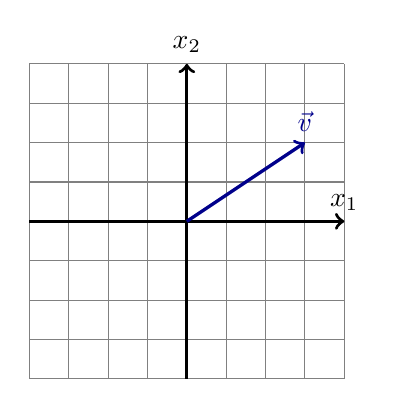
\begin{tikzpicture}[yscale=.5,xscale=.5] 
        \draw[gray](-4,-4) grid (4,4);  
        \draw[->,very thick]  (-4,0) -- (4,0) node[above]{$x_1$}; 
        \draw[->,very thick]  (0,-4) -- (0,4) node[above]{$x_2$}; 
        \draw[->,DarkBlue,very thick] (0,0) -- (3,2) node[above] {$ \vec v$}; 
    \end{tikzpicture}
    \end{center} 
\end{frame} 


\frame{\frametitle{Summary}

    \SummaryLine \vspace{4pt}
    \begin{itemize}\setlength{\itemsep}{8pt}

        \item orthogonal vectors and dot products
        \item orthogonal vectors and the Pythagorean Theorem
        \item sketching the set of vectors that are orthogonal to a given vector in $\mathbb R^2$
    
    \end{itemize}
    
    \vspace{8pt}
    \onslide<2->{A key concept in this video was that if $ \vec u$ and $ \vec v$ are \Emph{orthogonal}, then $ \vec u \cdot \vec v =0$, and 
    \begin{equation*}
    \lVert \vec u + \vec v \rVert ^2 =  \lVert \vec u  \lVert^2  +  \lVert  \vec v \rVert ^2
    \end{equation*}
    \vspace{12pt}
    This is an $n$-dimensional version of the Pythagorean Theorem. 
    }
}




